% Author: Hadrian Lau
% Website: https://www.hadrian.cc
% License: LaTeX Project Public License (LPPL)

\documentclass[a4paper,12pt]{article}

% Packages
\usepackage[utf8]{inputenc}
\usepackage[english]{babel}
\usepackage{amsmath, amsthm, amssymb, amsfonts}
\usepackage{graphicx}
\usepackage{setspace}
\usepackage{geometry}
\usepackage{float}
\usepackage{framed}
\usepackage[dvipsnames,svgnames]{xcolor}
\usepackage[most]{tcolorbox}
\usepackage{thmtools}
\usepackage{apacite}
\usepackage{indentfirst}
\usepackage{chemfig}
\usepackage{pgfplots}
\usepackage[version=4,arrows=pgf-filled,mathfontname=mathsf]{mhchem}
\usepackage{fancyhdr}
\usepackage{titlesec}
\usepackage{xpatch}
\usepackage{blindtext}
\usepackage{hyperref}
\usepackage{empheq}

% Settings
\pgfplotsset{width=15cm,compat=1.18}
\geometry{margin=1in}
\setstretch{1.5}
\newcommand{\HRule}[1]{\rule{\linewidth}{#1}}

% Box equations
\makeatletter
\newcommand{\colorboxed}[1]{\fcolorbox{DarkSeaGreen}{DarkSeaGreen!20}{\m@th$\displaystyle#1$}}
\xpatchcmd{\@Aboxed}{\boxed}{\colorboxed}{}{}
\makeatother

% Note sections
\makeatletter
\NewDocumentCommand{\mynote}{+O{}+m}{%
	\begingroup
	\tcbset{%
		noteshift/.store in=\mynote@shift,
		noteshift=1.5cm
	}
	\begin{tcolorbox}[nobeforeafter,
		enhanced,
		sharp corners,
		toprule=1pt,
		bottomrule=1pt,
		leftrule=0pt,
		rightrule=0pt,
		colback=DarkSeaGreen!20,
		#1,
		left skip=\mynote@shift,
		right skip=\mynote@shift,
		overlay={\node[right] (mynotenode) at ([xshift=-\mynote@shift]frame.west) {\textbf{Note:}} ;},
		]
		#2
	\end{tcolorbox}
	\endgroup
}
\makeatother

% Header and Footer
\pagestyle{fancy}
\fancyhf{}
\fancyhead[L]{Pendulum and Projectile Motion} % HERE
\fancyhead[R]{\thepage}

% Document
\begin{document}
	
	% Front page
	\title{ \normalsize \textsc{}
		\\ [2.0cm]
		\HRule{1.5pt} \\
		\LARGE \textbf{
			\uppercase{Pendulum and Projectile Motion} % HERE
			\HRule{2.0pt} \\ [0.6cm] 
			\LARGE{SPH3U Unit 1 Lab} % HERE
			\vfill
		}
	}
	\date{}
	\author{
		\textbf{Hadrian Lau Yiu Hei} \\ 
		DSC International School \\
		26th September, 2025\\ %HERE
		\href{https://hadrian.cc}{{\color{blue}\underline{\LaTeX\, document code}}}
	}
	\maketitle
	\thispagestyle{empty}
	
	\newpage
	
	% Table of content
	\setcounter{page}{1}
	\tableofcontents
	\newpage
	
	\section{Pendulum Motion}
	The purpose of the pendulum motion lab is to determine the acceleration due to gravity. A pendulum with a string length of 0.33m, attached with a 1.5cm in diameter steel ball, is dropped from a $5^\circ$ from the right without external forces. We recorded the time it takes for 10 oscillations for a total of 3 times for maximum accuracy. 
	
	\subsection{Raw data}
	Length of pendulum wire: $L=33\text{cm}=0.33\text{m}$\\
	
	
	This marginal time difference can be caused by errors like:
	\begin{itemize}
		\item Imprecise measurements: EXPLAIN
		\item Gross errors: EXPLAIN
	\end{itemize}
	
	\newpage
	
	\section{Projectile motion}
	The purpose of the projectile motion lab is to determine the properties of a projectile through displacement graphs, velocity graphs, and a variety of data. We placed a steel ball at the top of the ramp, and captured the trajectory of the steel ball using a slow motion camera.
	
	\subsection{Raw data}
	After reviewing the slow motion video, we can compile the following data points:
	\begin{center}
		\begin{tabular}{ |c|c|c| } 
			\hline
			$\vec{\Delta d_x}$ (m [$\rightarrow$]) & $\vec{\Delta d_y}$ (m [$\uparrow$]) & t (s)\\ 
			\hline\hline
			0.000m & 0.158m & 0.000s\\
			\hline 
			0.015m & 0.146m & 0.030s\\ 
			\hline
			0.030m & 0.128m & 0.060s\\
			\hline
			0.045m & 0.105m & 0.090s \\
			\hline
			0.060m & 0.068m & 0.120s\\
			\hline
			0.075m & 0.023m & 0.150s \\
			\hline
			0.083m & 0.000m & 0.165s\\
			\hline
		\end{tabular} 
	\end{center}

	\bigskip

	\mynote{We measured everything using the steel ball's center.}
	
	\newpage

	\begin{align*}
		\vec{\Delta d}_x&=\vec{\Delta d}_{xf}-\vec{\Delta d}_{xi}\\
		&=0.083 \text{m}\;[\rightarrow]-0.0 \text{m}\; [\rightarrow]\\
		\Aboxed{\vec{\Delta d}_x&=0.083\text{m}\; [\rightarrow]}
	\end{align*}

	\begin{center}
		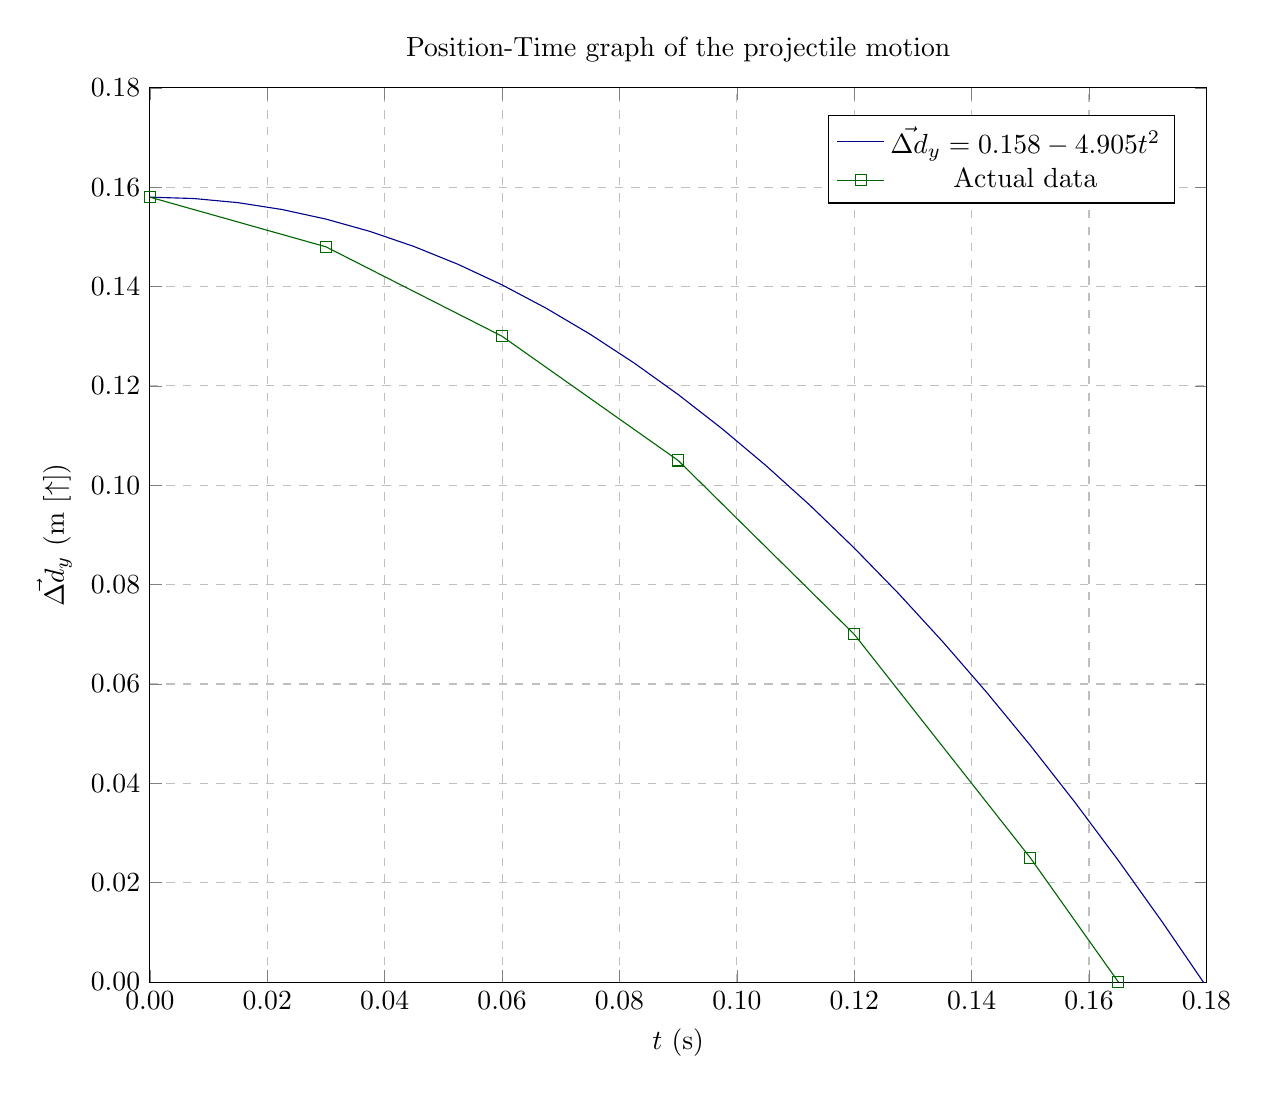
\begin{tikzpicture}
			\begin{axis} [
				title={Position-Time graph of the projectile motion},
				xlabel={$t$ (\text{s})},
				ylabel={$\vec{\Delta d}_y$ (\text{m} [$\uparrow$])},
				xmin=0, xmax=0.18,
				ymin=0, ymax=0.18,
				y tick label style={/pgf/number format/fixed,
					/pgf/number format/fixed zerofill={true}},
				x tick label style={/pgf/number format/fixed,
					/pgf/number format/fixed zerofill={true}},
				xtick distance=0.02,
				ytick distance=0.02,
				ymajorgrids=true,
				xmajorgrids=true,
				legend pos=north east,
				grid style=dashed,
			]	
				\addplot[
					color=DarkBlue,
					domain=0:0.18,
				] {
					0.158-4.905*x*x
				};
				\legend{$\vec{\Delta d}_y=0.158-4.905t^2$, Actual data}
				\addplot[
					color=DarkGreen,
					mark=square,
				] coordinates {
					(0,0.158)(0.03,0.148)(0.06,0.13)(0.09,0.105)(0.12,0.07)(0.15,0.025)(0.165,0)
				};
			\end{axis}
		\end{tikzpicture}
	\end{center}
	
	\section{Licensing}
	All LaTeX packages are provided by TeX Live under the LaTeX Project Public License (LPPL).\\
	The pgfplots package is licensed under the GNU General Public License (GPL) version 3 or later.\\
	The titlesec package is licensed under the MIT License.\\
	Template created by Hadrian Lau, derived from the HKUST Lab Report Template by Ma Wanqin, distributed under the Creative Commons CC BY 4.0 license.\\
	The LaTeX engine is provided by TeX Live under the LaTeX Project Public License (LPPL).\\
	NixOS Linux Operating System is distributed under the GNU Lesser General Public License (LGPL) version 2.1.\\
	The LaTeX code editor is provided by TeXstudio under the GNU General Public License (GPL) version 2.\\
	The LaTeX typesetting system is distributed under the LaTeX Project Public License (LPPL).\\
	
	%\newpage
	%\bibliographystyle{plain}
	%\bibliography{references}  % Add a .bib file if you have references
	
\end{document}

% All LaTeX packages are provided by TeX Live under the LaTeX Project Public License (LPPL).
% The pgfplots package is licensed under the GNU General Public License (GPL) version 3 or later.
% The titlesec package is licensed under the MIT License.
%
% Template created by Hadrian Lau, derived from the HKUST Lab Report Template by Ma Wanqin, distributed under the Creative Commons CC BY 4.0 license.
%
% The LaTeX engine is provided by TeX Live under the LaTeX Project Public License (LPPL).
% NixOS Linux Operating System is distributed under the GNU Lesser General Public License (LGPL) version 2.1.
% The LaTeX code editor is provided by TeXstudio under the GNU General Public License (GPL) version 2.
% The LaTeX typesetting system is distributed under the LaTeX Project Public License (LPPL).
